\documentclass{beamer}
\usepackage[utf8]{inputenc}

\usetheme{Madrid}
\usecolortheme{default}
\usepackage{amsmath,amssymb,amsfonts,amsthm}
\usepackage{txfonts}
\usepackage{multicol}
\usepackage{tkz-euclide}
\usepackage{listings}
\usepackage{adjustbox}
\usepackage{array}
\usepackage{tabularx}
\usepackage{gvv}
\usepackage{lmodern}
\usepackage{circuitikz}
\usepackage{tikz}
\usepackage{graphicx}

\setbeamertemplate{page number in head/foot}[totalframenumber]

\title
{4.2.8}
\date{September 20, 2025}
\author
{Aditya Mishra - EE25BTECH11005}

\begin{document}

\frame{\titlepage}

\begin{frame}{Question}
Find the direction and normal vectors of the line $5 = 2x$.
\end{frame}

\begin{frame}[fragile]
    \frametitle{Solution}
The equation of the line can be written as
\begin{align}
2x - 5 = 0
\end{align}

The slope of the line $x = \frac{5}{2}$ is undefined, therefore it can be expressed in the parametric form as:
\begin{align}
\myvec{x\\y} = \myvec{\tfrac{5}{2}\\0} + \lambda\myvec{0\\1}
\end{align}
\end{frame}

\begin{frame}[fragile]
    \frametitle{Solution}
Let $\myvec{x\\y}$ be the normal vector. Therefore
\begin{align}
\myvec{x\\ y}^T\myvec{0\\1} = 0 \\
y = 0\\
\myvec{x\\y} = \myvec{1\\0}
\end{align}
\end{frame}

\begin{frame}[fragile]
    \frametitle{Solution}
Therefore the line can be expressed as
\begin{align}
\myvec{1\\0}^Tx = \tfrac{5}{2}
\end{align}

\vspace{1cm}

Therefore, the direction vector is \myvec{0\\1}, and the normal vector is \myvec{1\\0}.
\end{frame}

\begin{frame}
\frametitle{Plot}
\begin{figure}[H]
    \centering
    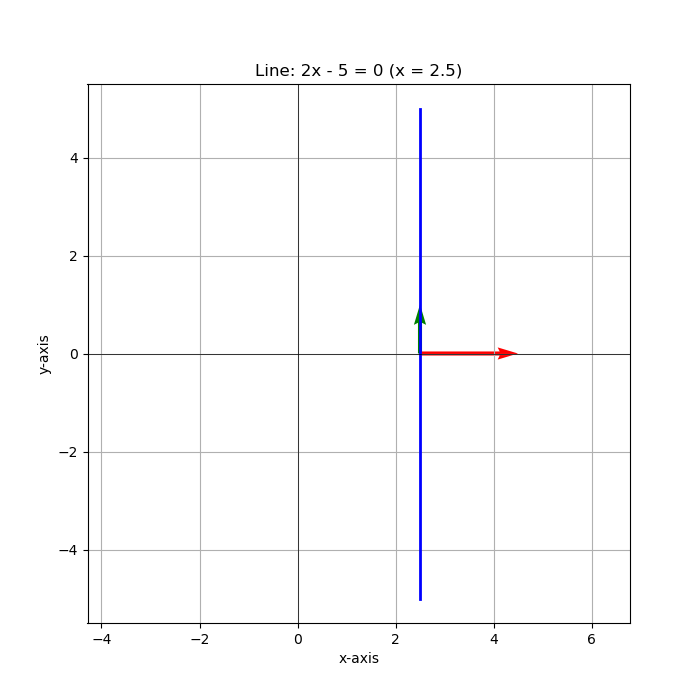
\includegraphics[width=0.6\columnwidth]{Figs/Figure_1.png}
    \caption{Plot of the line $x = 2.5$}
    \label{fig:428}
\end{figure}
\end{frame}

\begin{frame}
\frametitle{Code Repository}
The codes for this problem can be found at:

\centering
\url{https://github.com/Aditya-Mishra11005/ee1030-2025/tree/main/ee25btech11005/matgeo/4.2.8/Codes}
\end{frame}

\end{document}

